%%%%%%%%%%%%%%%%%%%%%%%%%%%%%%%%%%%%%%%%%%%%%%%%%%%%%%%%%%%%%%%
%
% Welcome to Overleaf --- just edit your LaTeX on the left,
% and we'll compile it for you on the right. If you open the
% 'Share' menu, you can invite other users to edit at the same
% time. See www.overleaf.com/learn for more info. Enjoy!
%
%%%%%%%%%%%%%%%%%%%%%%%%%%%%%%%%%%%%%%%%%%%%%%%%%%%%%%%%%%%%%%%

\documentclass{beamer}
%Information to be included in the title page:
\title{Predstavitev dela pri NRO}
\author{Ana Trstenjak}
\institute{Fakulteta za strojništvo, UL}
\date{2023}
\AtBeginSection[]
{
  \begin{frame}
    \frametitle{Kazalo}
    \tableofcontents[currentsection]
  \end{frame}
}

\begin{document}

\frame{\titlepage}
\begin{frame}
\frametitle{Kazalo vsebine}
\tableofcontents
\end{frame}

\section{Uvod}
\begin{frame}
\frametitle{Uvod}
Predstavitev je bila narejena kot del domače naloge v okviru izbirnega predmeta na Fakluteti za strojništvo.

  \frametitle{Uvod}

\begin{figure}
  
\includegraphics[width=0.3\linewidth]{ULFS logo.png}
    \caption{ULFS logo}
  \end{figure}
  \end{frame}


\section{Delovna orodja}
\begin{frame}
\frametitle{Delovna orodja}
Pri predmetu Napredna računalniška orodja smo uporabljali sledeča računalniška orodja:
\begin{itemize}
  \item MatLab
  \pause
  \item LaTeX
  \pause
  \item Beamer
\end{itemize}
\end{frame}

\section{Matlab}
\begin{frame}
\frametitle{Matlab}
V okviru prve domače naloge smo imeli nalogo, da v okolju Matlab predstavimo kako se izračuna približek števila $\pi$ s pomočjo metode Monte Carlo.

Primerjali smo ploščino kroga in njemu očrtanega kvadrata, ter gledali ali je naključno generirana točka zunaj ali znotraj kvadrata.
\end{frame}

\section{GitHub}
\begin{frame}
\frametitle{GitHub}
GitHUb je platforma za gostovanje in upravljanje različnih projektov programske opreme s sistemom nadzora različic Git. Preko Git-a lahko nadzorujemo različice, kar nam omogoča sodelovanje med razvijalci.Spremembam lahko sledimo v zgodovini, ki jo Git shranjuje.

Na spodnji strani lahko vidimo posnetek zaslona na mojem repozitorijo na GitHubu.

\begin{figure}
  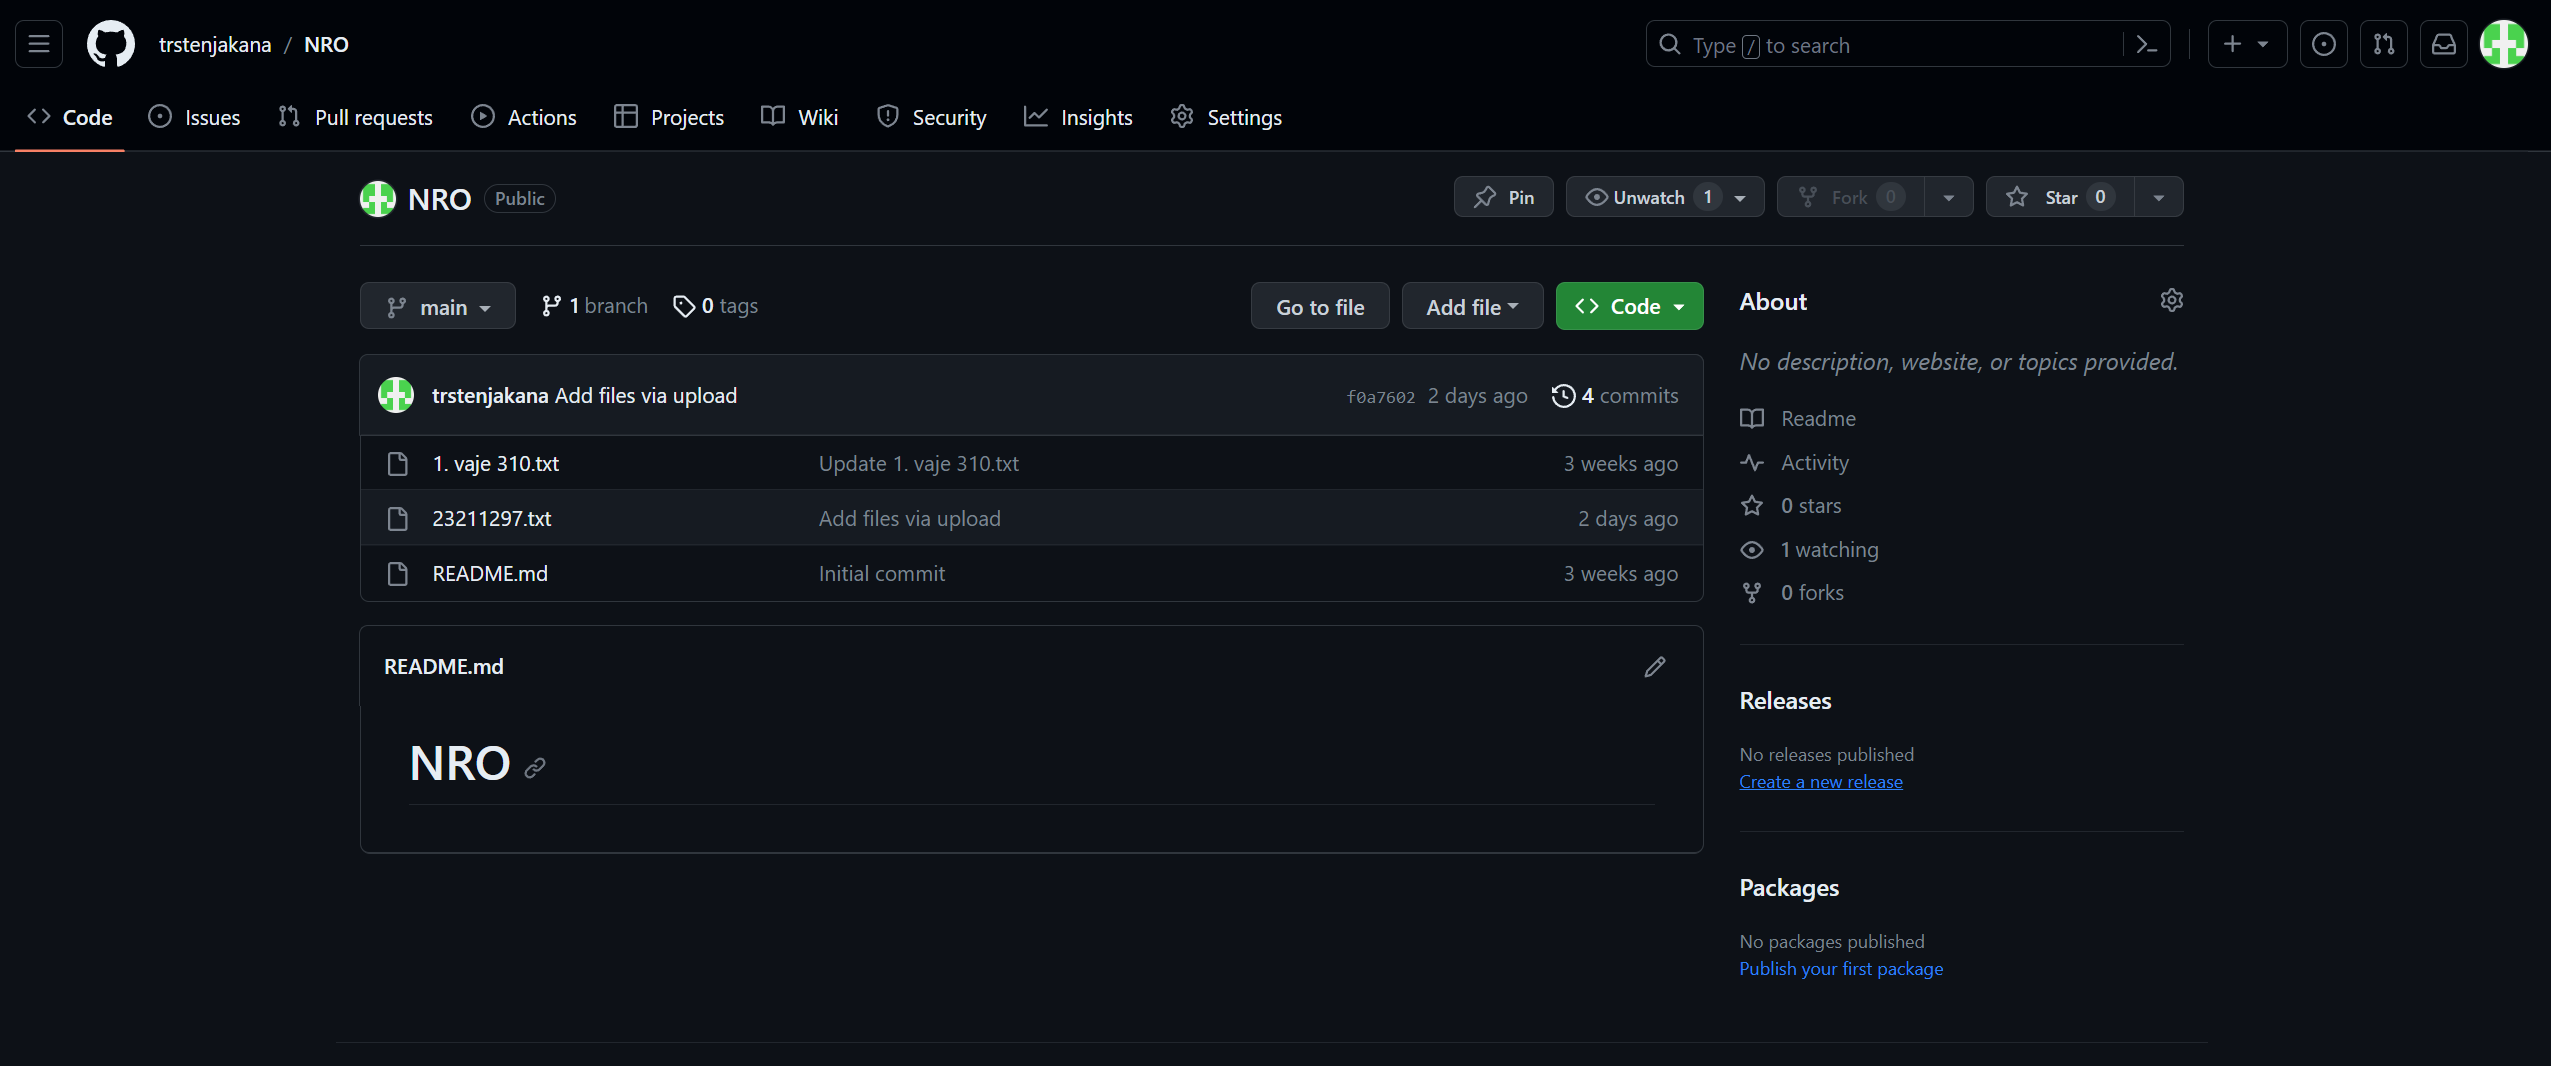
\includegraphics[width=0.7\linewidth]{GitHub.png}
    \caption{Github repozitorij NRO}
  \end{figure}
\end{frame}
\section{LaTeX}
\begin{frame}
    \frametitle{LaTeX}
    LaTeX je besedilni prejevalnik, ki nam omogoča urejanje kompleksnih dokumentov. Osebno uporabljam Overleaf, ki je brezplačen in ne potrebujemo ničesar naložiti na računalnik.
    Prednosti LaTeX-a:
    \begin{itemize}
        \item Enostavno pisanje matematičnih enačb
        \item Več avtorjev na istem projektu
        \item Zanesljivost
        \item Citiranje in navajanje referenc
        \item Brezplačen
        \item Prilagodljivost
        \item in še mnoge druge ... 

    \end{itemize}
\end{frame}
\section{Zaključek}
\begin{frame}{Zaključek}
    V okviru prve domače naloge smo se naučili uporabljati Matlab, Beamerja(Overleaf) in GitHuba.
    
\end{frame}
\end{document}

\end{document}  
\end{frame}
\end{document}